\documentclass[10pt,a4paper]{article}
\usepackage[utf8]{inputenc}
\usepackage[german]{babel}
\usepackage{amsmath}
\usepackage{amsfonts}
\usepackage{amssymb}
\usepackage[left=2cm,right=2cm,top=2cm,bottom=2cm]{geometry}

\usepackage{graphicx}
\usepackage{caption}
\usepackage[colorlinks]{hyperref}



\author{Christian Bespin \and Christopher Deutsch}
\title{Übungsblatt 1: Numerische Methoden der Physik}
\begin{document}
\maketitle

\section{Madelung-Konstante des NaCl-Kristalls}
\subsection{Physikalischer Hintergrund}
In einem Kristallgitter sind die Ionen durch elektrostatische Wechselwirkung
untereinander an den Kristall gebunden. Uns interessiert die durchschnittliche
potentielle Energie eines dieser Ionen (wird mit dem Index $i$ bezeichnet).
Diese entsteht in erster Näherung aus der Überlagerung der Coulomb-Potentiale
der Punktladungen im Kristallgefüge
(werden mit dem Index $j$ bezeichnet). Die Ladungszahl des jeweiligen Ions sei $z$
und $r_{ij}$ ist der Abstand des betrachteten Ionenpaars. Wir summieren für
jedes Ion des Kristalls (mit Ausnahme des $i$-Ions, da dessen Potential auf sich
selbst keinen Einfluss hat) den Beitrag zum Potential:

\begin{align}
\label{EPot}
E_G = \sum_{j\atop i \neq j} \frac{1}{4 \pi \epsilon_0}
\frac{z_i e \cdot z_j e}{r_{ij}}
\end{align}
Erweitern der Gleichung (\ref{EPot}) mit dem Gitterabstand $a$ und
Zusammenfassen des Faktors in die durchschnittliche Energie eines Ionenpaars
$E_P$ mit Abstand $a$ ergibt:

\begin{align}
E_G = \frac{1}{4 \pi \epsilon_0} \frac{e^2}{a} \sum_{j\atop i \neq j}
\frac{z_i z_j}{r_{ij}/a} = E_P \sum_{j\atop i \neq j} \frac{z_i z_j}{r_{ij}/a}
\end{align}
Schließlich wird die Geometrie des Kristalls in der Madelung-Konstante
zusammengefasst:

\begin{align}
\label{Madelungkonstante}
\alpha = \frac{E_G}{E_P} = \sum_{j\atop i \neq j} \frac{z_i z_j}{r_{ij}/a}
\end{align}
Dabei ist $r_{ij}/a$ der mit der Gitterkonstanten normalisierte Abstand der Ionen,
welcher im Folgenden ausschließlich für Längen verwendet wird.

\subsection{Algorithmus im 3-dimensionalen Fall}
\subsubsection{Struktur von Natriumchlorid}

Die nächsten Nachbarn eines jeden Ions sind sechs Ionen entgegengesetzter
Ladung. Diese Ionen befinden sich an den Eckpunkten eines regelmäßigen
Oktaeders. Dadurch kann das Vorzeichen der Ladung an der Gitterstelle
$\mathbf{r} = \left( x,y,z \right)$ relativ zu einer anderen Ladung durch:
\begin{align}
\mathrm{sgn}\left(z(\mathbf{r})\right) = \pm \left( -1 \right)^{x+y+z}
\label{eq:vorzeichen}
\end{align}
berechnet werden. Dabei wird das Vorzeichen so gewählt, dass dieses mit der Ladung
des Referenz-Ions übereinstimmt (Na: $+$; Cl: $-$). Diese Tatsache
äußert sich auch darin, dass das Vorzeichen der Madelung-Konstante vom
betrachteten Ion abhängt (generell: $\alpha_{Na} = - \alpha_{Cl}$).
\subsubsection{Probleme der naiven Methode}

Zunächst wurde die naive Implementierung analog zur mathematischen Beschreibung
getestet. Dabei wurde die Madelung-Konstante für einen Würfel analog zu
Gl. (\ref{Madelungkonstante}), über sukzessive Erweiterung des Würfels um eine
Schale berechnet. Es fällt schnell die schlechte Konvergenz auf, die sich
physikalisch darin manifestiert, dass der Kristall, beim einfachen Erweitern
mit einer Schale, nicht elektrisch neutral bleibt. Dieses Problem wurde von Evjen
\cite{Evjen} gelöst, indem er den Kristall in elektrisch neutrale Elementarzellen
aufteilt, die einen flacheren Potentialverlauf haben als einzelne Punktladungen.
Eine solche Zelle ist in Abbildung \ref{skalierungsgrafik3d} dargestellt,
dabei sind die gebrochenen Ladungen durch das Überlappen von mehreren Elementarzellen
motiviert (vgl. Abb. \ref{zellensumme} für das zweidimensionale Analogon). Die Summe über 
alle Elementarzellen eines Würfels resultiert darin, dass die Ecken des Würfels
$\frac{1}{8}$, Kanten $\frac{1}{4}$ und Seitenflächen $\frac{1}{2}$ gewichtet werden
und der Innenraum voll in die Gewichtung eingeht.

\begin{figure}[h]
	\centering
	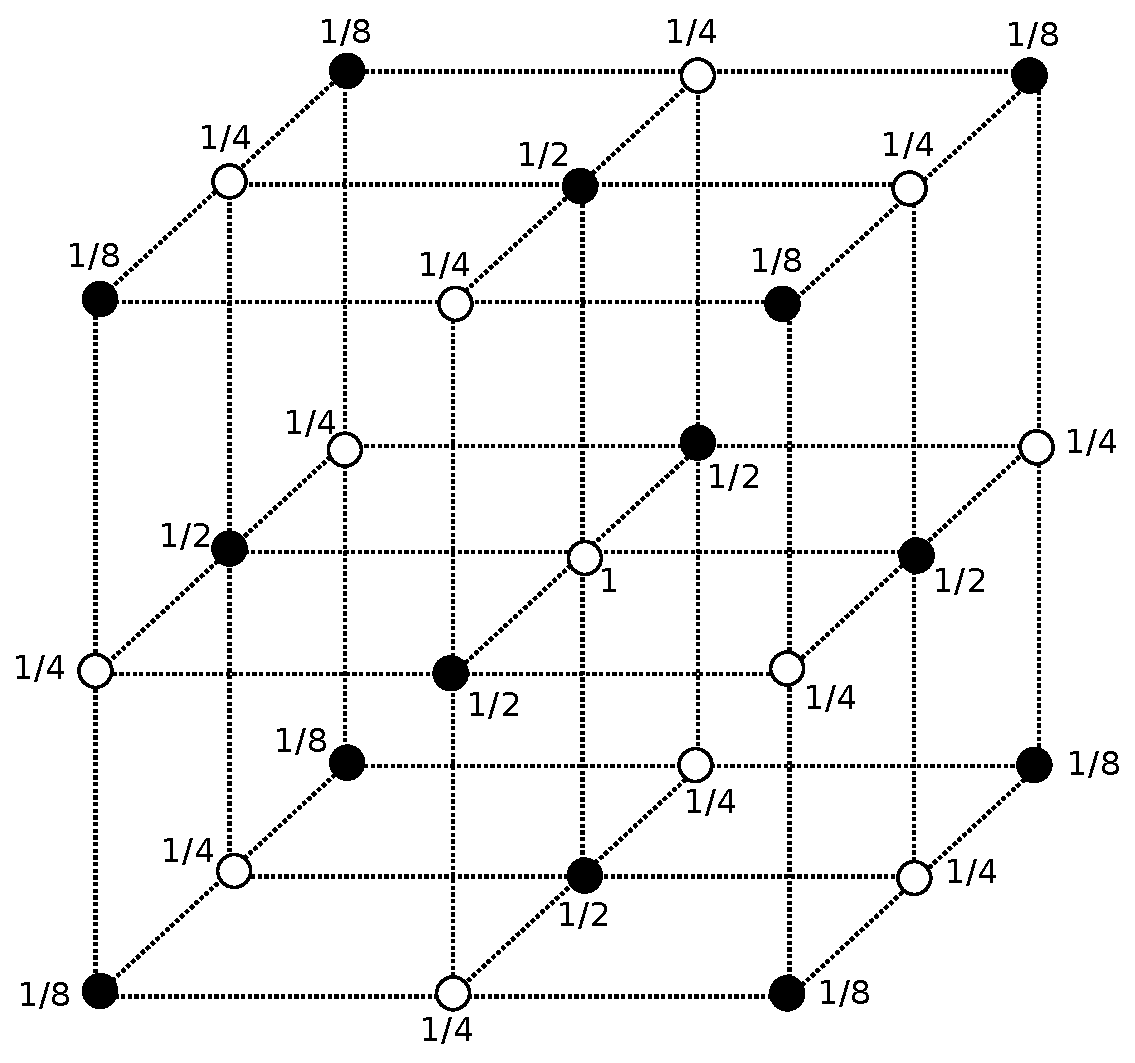
\includegraphics[scale = 0.35]{./figures/wuerfel.eps}
	\caption{neutrale Elementarzelle nach Evjen}
	\label{skalierungsgrafik3d}
\end{figure}

\subsubsection{Beschreibung}

Der verwendete Algorithmus beginnt mit einem Ion im Koordinatenursprung. Dieses
erweitern wir schrittweise um eine Schale von Ionen mit den Ladungenzahlen gemäß
Gl. (\ref{eq:vorzeichen}). Wir nutzen nun die Symmetrie des Würfels, um den Beitrag
der so konstruierten Schale zur Madelung-Konstante zu berechnen. Dazu teilen wir die
Schale in 8 äquivalente Ecken, 12 Kanten und 6 Seitenflächen auf, berechnen für
jeweils eines dieser Objekte den Beitrag zur Madelung-Konstante (nach Evjen gewichtet)
und multiplizieren mit dem entsprechenden Faktor. Dabei ist zu beachten, dass wir
den Rest der Gewichtung zwischenspeichern müssen, da nach dem Hinzufügen der nächsten
Schale die Ionen im Inneren des Würfels voll gewichtet werden (bei der nächsten Schale
wird dann einfach der Rest auf die Madelung-Konstante addiert). Diese Vorgehensweise ist notwendig, da wir das Verfahren solange wiederholen, bis die Differenz der Madelungkonstante
von zwei aufeinanderfolgenden Schalen kleiner als eine Zahl $0 < \epsilon < 1$ wird. Die
mathematische Relevanz dieser Abbruchbedingung wird in Abschnitt \ref{sssec:Konvergenz}
erklärt.

\subsubsection{Konvergenz}

\label{sssec:Konvergenz}
\begin{figure}[h]
\begin{minipage}[c]{0.5\textwidth}
\begin{center}
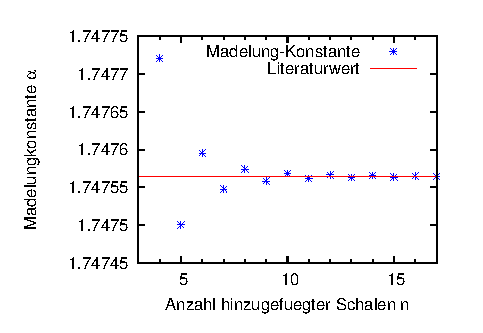
\includegraphics[width=\textwidth]{./figures/ergebnis.eps}
\captionof{figure}{Konvergenz des 3D Dingens}
\label{plotkonvergenz3d}
\end{center}
\end{minipage}
\begin{minipage}[c]{0.5\textwidth}
\begin{center}
\begin{tabular}{c|c|c}
\rule[-1ex]{0pt}{2.5ex} $n$ & $\alpha$ & $\delta$ \\ 
\hline 
\rule[-1ex]{0pt}{2.5ex} $1$ & $1.456029925630$ & $1.67\cdot10^{-1}$ \\ 
\hline 
\rule[-1ex]{0pt}{2.5ex} $2$ & $1.751769133337$ & $2.41\cdot10^{-3}$ \\ 
\hline
\rule[-1ex]{0pt}{2.5ex} $5$ & $1.747500502341$ & $3.67\cdot10^{-5}$ \\ 
\hline 
\rule[-1ex]{0pt}{2.5ex} $10$ & $1.747568603772$ & $2.29\cdot10^{-6}$ \\ 
\hline 
\rule[-1ex]{0pt}{2.5ex} $20$ & $1.747564845218$ & $1.43\cdot10^{-7}$ \\ 
\hline 
\rule[-1ex]{0pt}{2.5ex} $50$ & $1.747564601048$ & $3.67\cdot10^{-9}$ \\
\hline
\rule[-1ex]{0pt}{2.5ex} $100$ & $1.747564595034$ & $2.30\cdot10^{-10}$ \\ 
\hline
\rule[-1ex]{0pt}{2.5ex} $200$ & $1.747564594660$ & $1.51\cdot10^{-11}$ \\ 
\hline
\rule[1ex]{0pt}{2.5ex} Lit. & $1.747564694633$ & $ - $
\end{tabular}
\captionof{table}{Konvergenz}
\end{center}
\end{minipage}
\end{figure}

Wie man in der Tabelle sehen kann konvergiert die Evjen-Methode sehr schnell
gegen den Literaturwert $\alpha_{NaCl} = 1.7475646946331822$ \cite{Sakamoto}.
Der nach unserer Methode berechnete Wert alterniert, wie man der Abbildung
entnehmen kann, stets mit fallender Amplitude um den wahren Wert. Dies
rechtfertigt unser Abbruchkriterium, denn der wahre Wert liegt offenbar
näher am letzten Datenpunkt als die Differenz zum Vorletzten. So ist garantiert,
dass bei Eintreten der Abbruchsbedingung der absolute Fehler des berechneten
Wertes kleiner als $\epsilon$ ist.

\subsection{Algorithmus im 2-dimensionalen Fall}
\subsubsection{Beschreibung}
Um die Methode von Evjen auf den zweidimensionalen Fall zu übertragen, sieht man leicht,
dass um elektrische Neutralität einer Elementarzelle zu erreichen, die Ecken mit $\frac{1}{4}$
und die Kanten mit $\frac{1}{2}$ gewichtet werden müssen (Abbildung \ref{skalierungsgrafik2d}).
Die Summe über alle Elementarzellen führt analog zum 3-dimensionalen Fall dazu, dass die Ecken
des Quadrates $\frac{1}{4}$ und die Kanten $\frac{1}{2}$ (siehe Abbildung \ref{zellensumme}).
Die Vorgehensweise ist analog zum 3-dimensionalen Fall, mit Ausnahme der Abbruchbedingung.
Der Wert der Madelungkonstante alterniert in diesem Fall nicht um den wahren Wert, weshalb
wir einen direkten Vergleich mit dem Literaturwert durchführen. Die Funktion wird beendet
sobald absolute Fehler einen vorgegebenen Wert unterschreitet.


\begin{minipage}[c]{0.5\textwidth}
\begin{center}
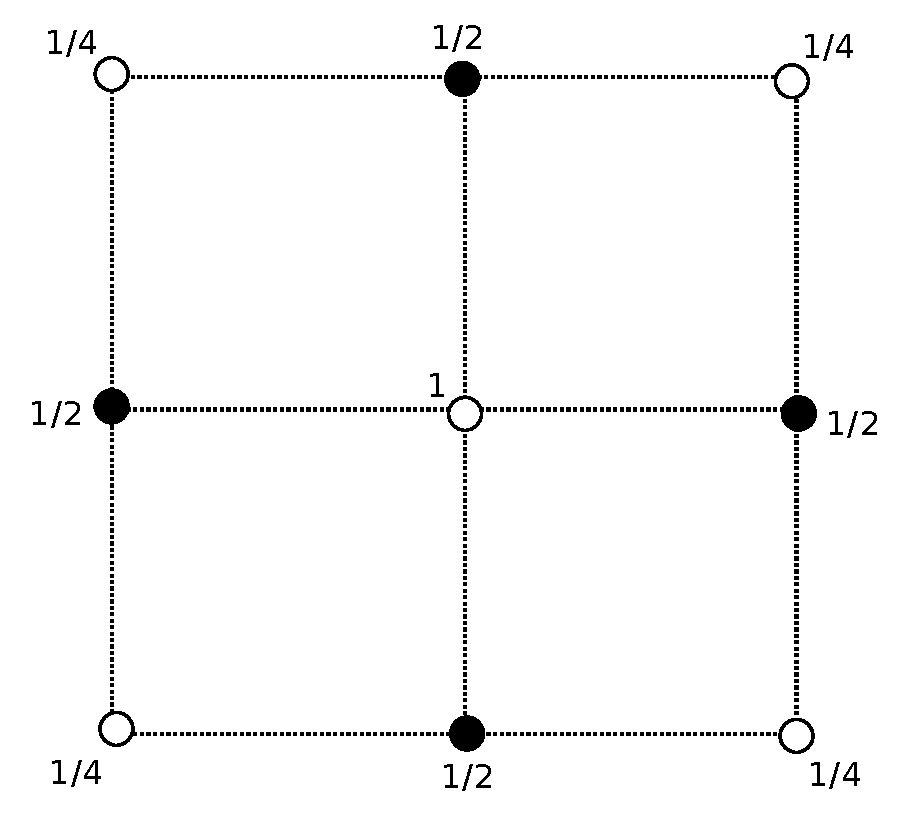
\includegraphics[height=0.65\textwidth]{./figures/quadrat.eps}
\captionof{figure}{neutrale Elementarzelle (2-dim.)}
\label{skalierungsgrafik2d}
\end{center}
\end{minipage}
\begin{minipage}[c]{0.5\textwidth}
\begin{center}
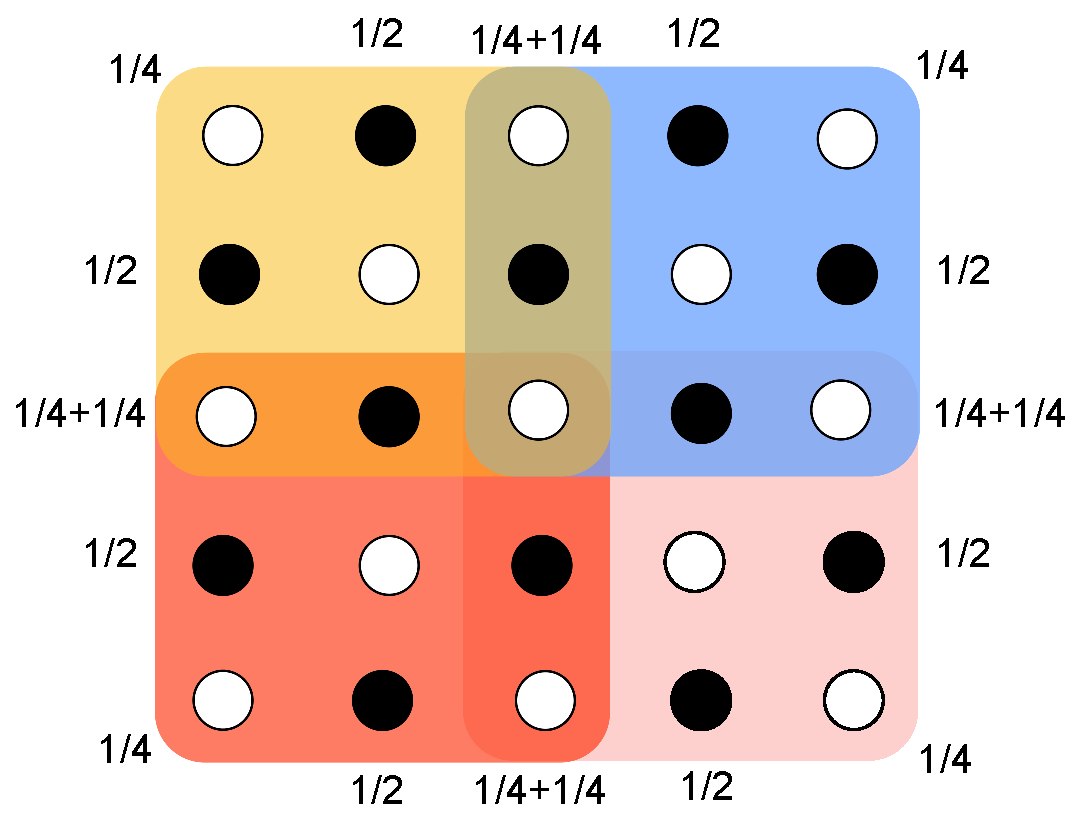
\includegraphics[height=0.65\textwidth]{./figures/elementarzelle.eps}
\captionof{figure}{Aneinanderreihung von Elementarzellen}
\label{zellensumme}
\end{center}
\end{minipage}
	

\subsubsection{Konvergenz}

Wie gut konvergiert der 2-dimensionale Algorithmus.
$\alpha = 1.6155426267128247$ \footnote{\href{https://oeis.org/A088537}{A088537} \emph{Decimal expansion of Madelung's constant M2} The On-Line Encyclopedia of Integer Sequences}.

\subsection{Fazit}

Verwendeter Literaturwert  .


\begin{thebibliography}{9}

\bibitem{Evjen}
Evjen, H. M.
\emph{On the Stability of Certain Heteropolar Crystals},
Physical Review Letters \textbf{39},
675-687 (1932)

\bibitem{Sakamoto}
Sakamoto, Y.
\emph{Madelung Constants of Simple Crystals Expressed in Terms of Born's Basic
Potentials of 15 Figures},
The Journal of Chemical Physics \textbf{28},
164 (1958)

\end{thebibliography}

\end{document}
